% The project can be found at 
% https://github.com/dev-aditya/LaTeX-template


\documentclass{package/notes}

%%%%%%%%%% Default Package %%%%%%%%%%%%%
\usepackage{package/color-env}
%%%%%%%%%% %%%%%%%%%%%%%%% %%%%%%%%%%%%%

%%%%%%%%%% Required Packages %%%%%%%%%%%%%
% \usepackage{background}
\usepackage[object=vectorian]{pgfornament} %% used in title.tex
\usepackage{calligra} %%% (optional) to make the Title text beautiful 

%%%%%% Optional Packages %%%%%%%
\usepackage{lettrine} %% for nice looking 
\usepackage{GoudyIn} %% first Letter of the paragraph
%%%%%%%%%%%%%%%%%%%%%%%%

\usepackage{lipsum}  %% for dummy text 
\usepackage{amssymb,amsmath,amsfonts}  %%% for maths
%%%%%%%%%%%%%%%%%%%%%%%%%%%%%%%%%%%%%
\usepackage{subcaption} %% for subfigures

%%%%%%%%%%%%%%%%%%%%%%%%%%%%%%%%%%%%%
\renewcommand{\LettrineFontHook}{\color{black}\GoudyInfamily{}}
\LettrineTextFont{\itshape}
\setcounter{DefaultLines}{3}%
%%%%%%%%%%%%%%%%%%%%%%%%%%%%%%%%%%%%%

%%%% Bibliography %%%%%%%%%
% Required packages are included in notes class
% Can be tweaked in the notes.cls file itself

\addbibresource{resource/references.bib}

% \includeonly{package/title-page.tex, chapters/2FirstOrderDifferentials.tex}

\begin{document}

\newpage

\begin{titlepage}

  %%%%%%%%%%%%%%%%%%%%%%%%%%%%%%%%%%%% Inspired From  %%%%%%%%%%%%%%%%%%%%%%%%%%%%%%%%%%%%%%%%%%%%%%%%% 
  %%%%  https://www.reddit.com/r/LaTeX/comments/j9d739/hello_world_in_latex_is_a_lot_cooler/   %%%%%
  %%%%%%%%%%%%%%%% If this doesn't look nice then you may remove it %%%%%%%%%%%%%%%%%%%%%%%%%%
  
  \backgroundsetup{
  scale=1,
  opacity=1,
  angle=0,
  color=black,
  contents={
  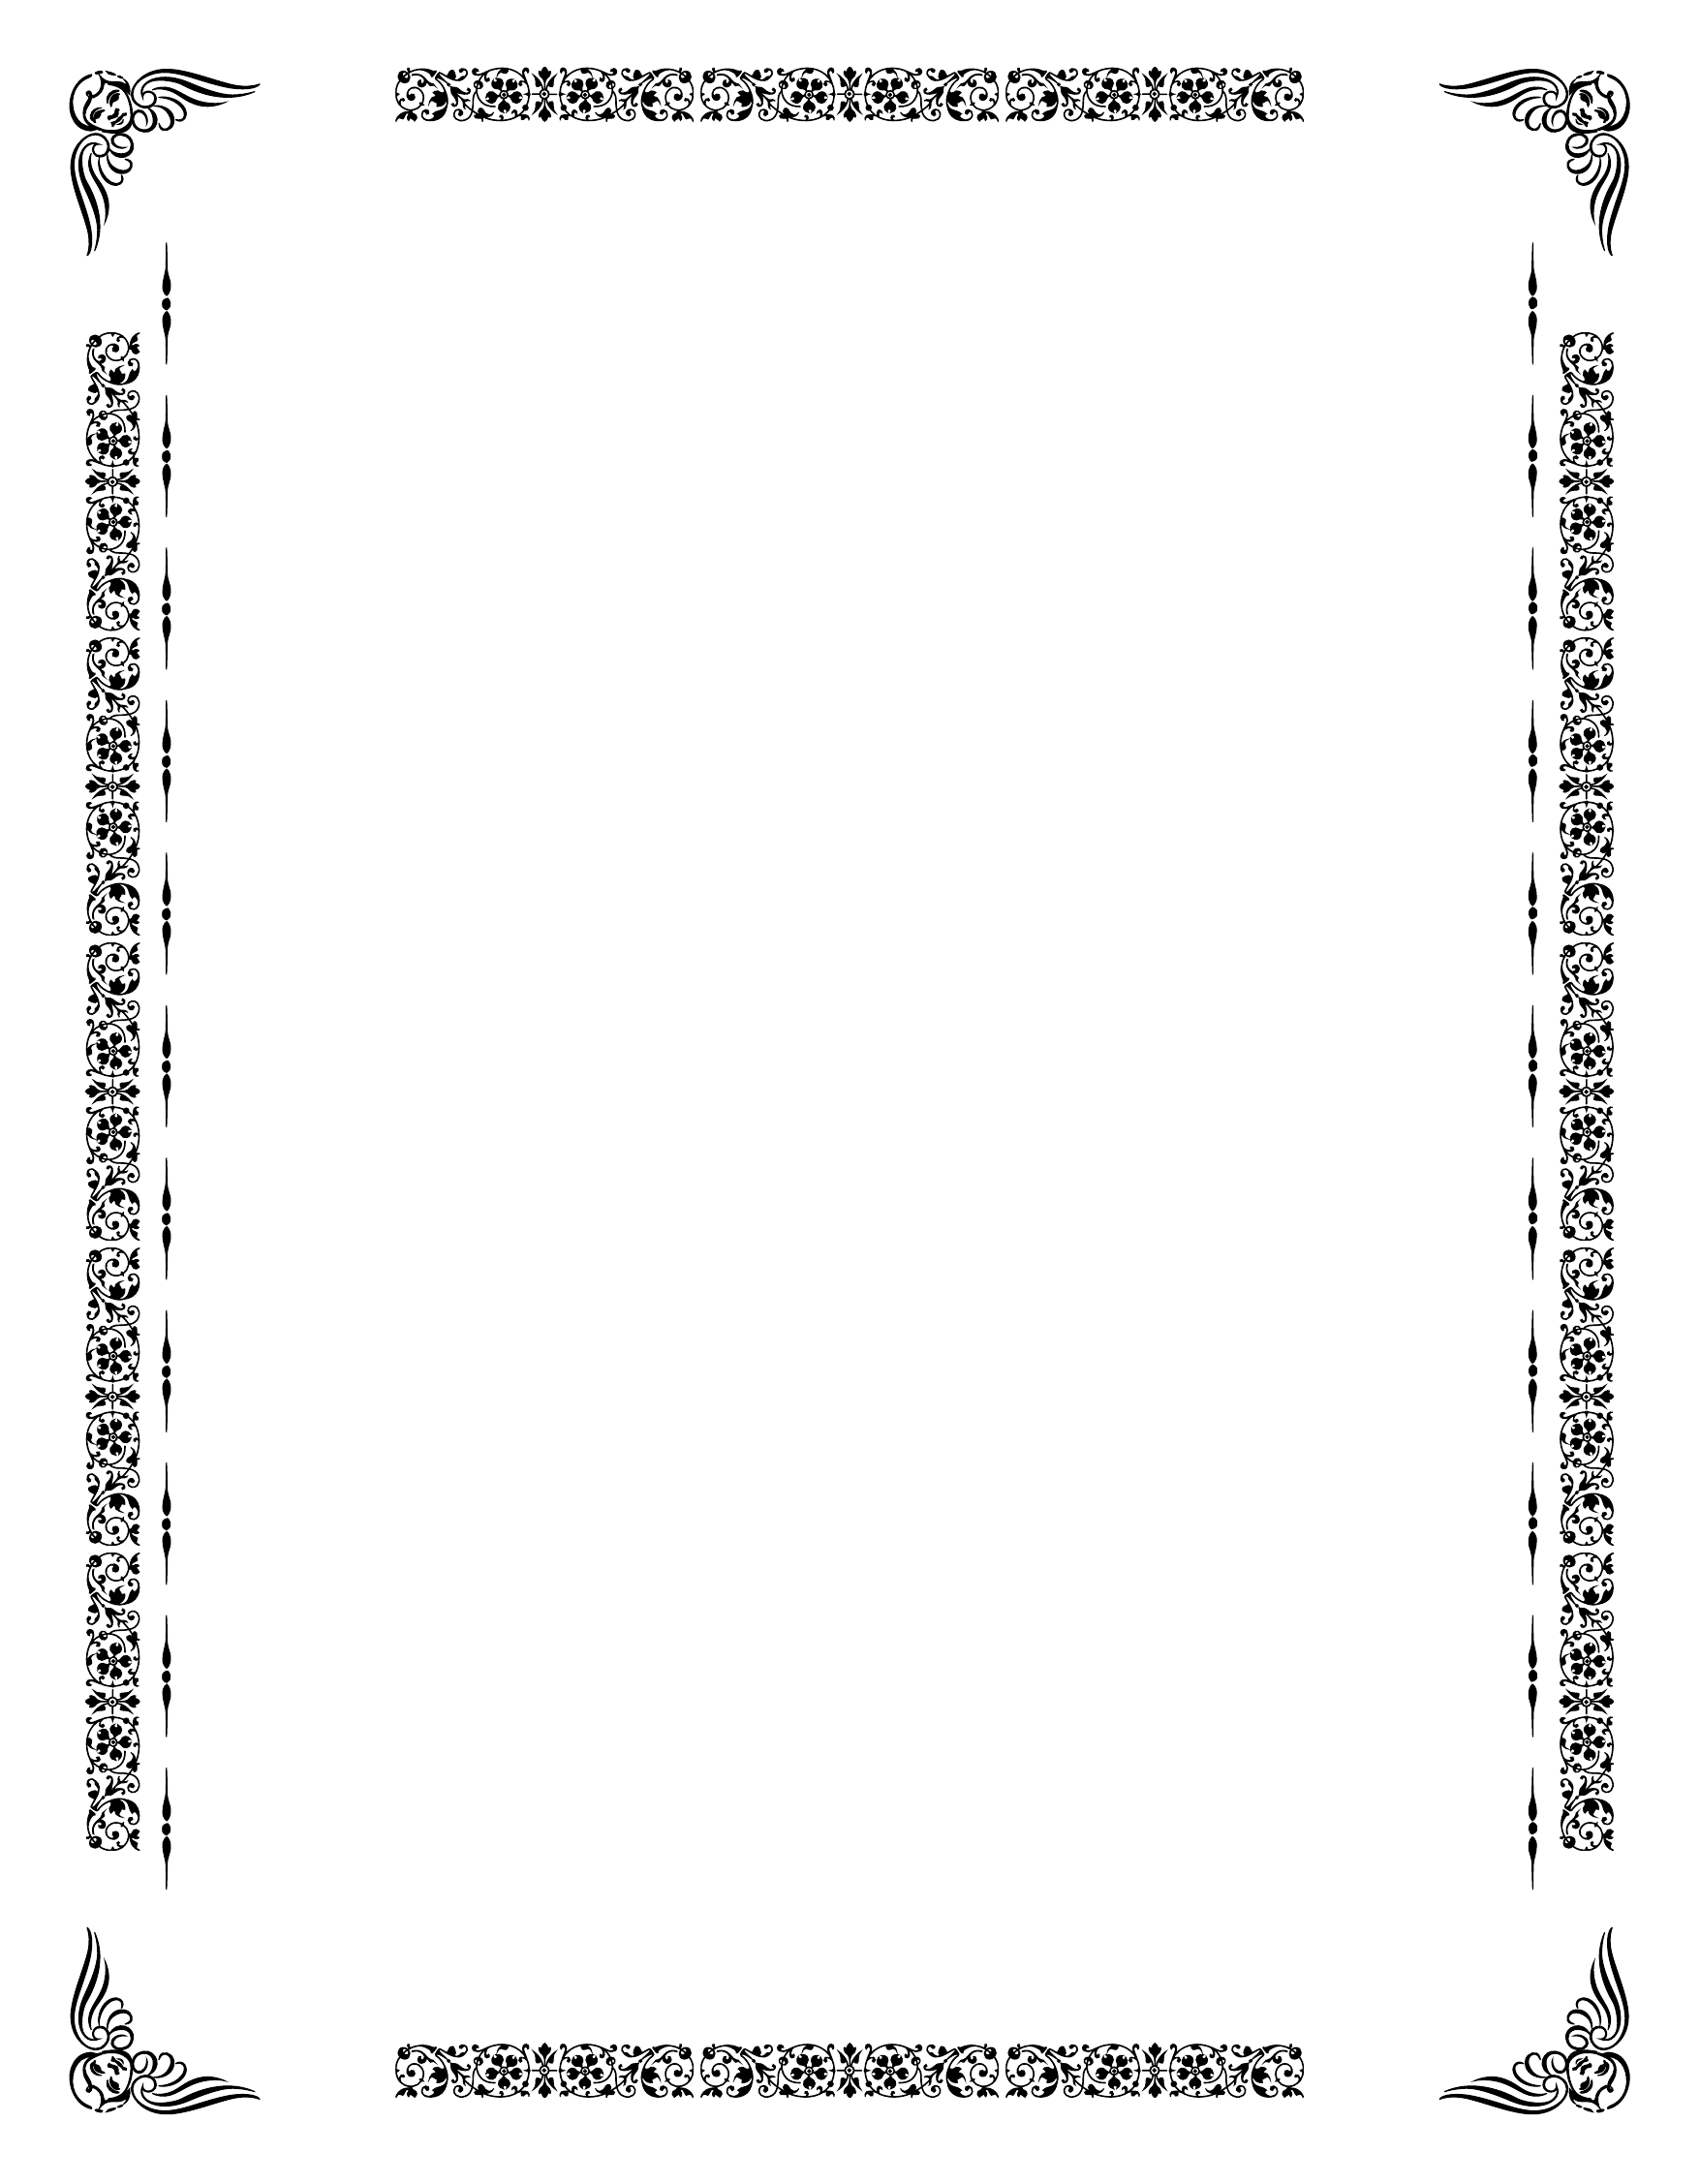
\begin{tikzpicture}[color=black, every node/.style={inner sep= 15pt}]
  \node (NW) [anchor=north west] at (current page.north west){\pgfornament[width=2.5cm] {131}};
  \node (NE) [anchor=north east] at (current page.north east){\pgfornament[width=2.5cm, symmetry=v]{131}};
  \node (SW) [anchor=south west] at (current page.south west){\pgfornament[width=2.5cm, symmetry=h]{131}};
  \node (SE) [anchor=south east] at (current page.south east){\pgfornament[width=2.5cm, symmetry=c]{131}};
  \foreach \i in {-4,0,4}
  \node[anchor=north,xshift=\i cm] at (current page.north){\pgfornament[scale=0.25,symmetry=v]{71}};
  \foreach \i in {-4,0,4}
  \node[xshift=\i cm, yshift=32.25 pt] at (current page.south){\pgfornament[scale=0.25,symmetry=v]{71}};
  \foreach \i in {-8,-4,0,4,8}
  \node[yshift=\i cm, xshift=32.25pt, rotate=90] at (current page.west){\pgfornament[scale=0.25,symmetry=v]{71}};
  \foreach \i in {-8,-4,0,4,8}
  \node[yshift=\i cm, xshift=-32.25pt, rotate=90] at (current page.east){\pgfornament[scale=0.25,symmetry=v]{71}};
  \foreach \i in {-11,-9,...,7,9}
  \node[anchor=west, yshift=\i cm, xshift=52.25pt, rotate=90] at (current page.west){\pgfornament[scale=0.1]{80}};
  \foreach \i in {-11,-9,...,7,9}
  \node[anchor=east, yshift=\i cm, xshift=-52.25pt, rotate=-90] at (current page.east){\pgfornament[scale=0.1]{80}};
  \end{tikzpicture}
  }}
  
  %%%%%%%%%%%%%%%%%%%%%%%%%%%%%%%%%%%%%%%%%%%%%%%%%%%%%%%%%%%%%%%%%%%%%%%%%%%%%%%%%%%%%%%%%%%%%%%%%%%%%%%%%%%%%%%%%%
  
  \centering % Centre everything on the title page
      
  \scshape % Use small caps for all text on the title page
  
  \vspace*{\baselineskip} % White space at the top of the page
  
  %------------------------------------------------
  %	Title
  %------------------------------------------------
  
  \rule{\textwidth}{1.6pt}\vspace*{-\baselineskip}\vspace*{2pt} % Thick horizontal rule
  \rule{\textwidth}{0.4pt} % Thin horizontal rule
  
  \vspace{0.75\baselineskip} % Whitespace above the title
  
  {\huge \calligra{ Applied Linear Algebra }\\} % Title
  
  \vspace{0.75\baselineskip} % Whitespace below the title
  
  \rule{\textwidth}{0.4pt}\vspace*{-\baselineskip}\vspace{3.2pt} % Thin horizontal rule
  \rule{\textwidth}{1.6pt} % Thick horizontal rule
  
  \vspace{2\baselineskip} % Whitespace after the title block
  
  %------------------------------------------------
  %	Subtitle
  %------------------------------------------------
  
  \LARGE{MATH363} 
  
  \vspace*{3\baselineskip} % Whitespace under the subtitle
  
  
  
  \vspace{0.5\baselineskip} 
  
  {\scshape   \LARGE Dr. McKenzie\\ } % Editor list
  
  \vspace{0.2\baselineskip} 
  
  \textit{\Large Gonzaga University} 
  
  \vfill 
  
  %------------------------------------------------
  % Author
  %------------------------------------------------
  
  \begin{figure}[!h]
      \centering
      
\includegraphics[width = 4cm, height= 3cm]{resource/images/Gonzaga_University_Logo.jpg}%% include the university icon here
  \end{figure}
  \vspace{0.3\baselineskip} 
  
  
  {\large Edited by\\  Cameron Williamson}
  \end{titlepage}
\tableofcontents

\include{chapters/Definitions.tex}
\include{chapters/Theorems.tex}
\chapter{Introduction to Ordinary Differential Equations}

Differential equations come from real-world problems and problems in applied mathematics. When mathematics is applied to real-world problems, it is often the case that finding a relation between a function and its rate of change is easier than finding a formula for the function itself; it is this relation between an unknown function and its derivatives that produces a differential equation.\newline
To give a very simple example, a biologist studying the growth of a population with size at time $t$ given by the function $P(t)$, might make the very simple, but logical, assumption that a population grows at a rate directly proportional to its size. In mathematical notation, the equation for $P(t)$ could then be written as:

\[
  \frac{dp}{dt} = rP(t)
\]

Where the constant of proportionality, $r$ would probably be determined experimentally by biologists working in the field. Equations used for modeling population growth can be much more complicated than this, sometimes involving scores of interacting populations with different properties.

\section{Basic Terminology}

  \begin{definition}
    A differential equation is any equation involving an unknown function and one or more if its derivatives.
  \end{definition}

  The following are examples of differential equations:

    \begin{enumerate}
      \item $P'(t)=rP(t)(1-P(t)/N)-H$ harvested population growth
      \item $\frac{d^2x}{d\tau^2}+0.9\frac{dx}{d\tau}+2x=0$ spring mass equation
      \item $I''(t)+4I(t)=sin(\omega t) $ RCL circuit showing beats
      \item $y''(t) + \mu(y^2(t)-1)y'(t)+y(t)$ ban der Pol equation
      \item $\frac{\partial^2}{\partial x^2}u(x,y)+\frac{\partial^2}{\partial y^2}u(x,y) = 0$ Laplace's equation
    \end{enumerate}

  \subsection{Ordinary vs. Partial Differential Equations}

    Differential equations fall into two very broad categories, called ordinary differential equations and partial differential equations. If the unknown function in the equation is a function of only one variable, the equation is called an ordinary differential equation. If the unknown function in the equation depends on more than one independent variable, the equation is called a partial differential equation, and in this case, the derivatives appearing in the equation will be partial derivatives.

  \subsection{Independent Variables, Dependent Variables, and Parameters}

   Three different types of quantities can appear in a differential equation. The unknown function, for which the equation is to be solved, is called the dependent variable, and when considering ordinary differential equations, the dependent variable is a function of a single independent variable. In addition to the independent and dependent variables, a third type of variable, called a parameter, may appear in the equation. A parameter is a quantity that remains fixed in any specification of the problem, but can very from problem to problem.
  
  \subsection{Order of a Differential Equation}

    Another important way in which differential equations are classified is in terms of their order.

    \begin{definition}
      The order of a differential equation is the order of the highest derivative of the unknown function that appears in the equation.
    \end{definition}

    The differential equation 1 is a first-order equation and the others are all second-order. Even though equation 5 is a partial differential equation, it is still said to be of second order since no derivatives of order higher than two appear in the equation.

  \subsection{What is a solution}

    Given a differential equation, what is a solution? We must realize that we are looking for a function, and therefore it needs to be defined on some interval of its independent variable.

    \begin{definition}
      An analytic solution of a differential equation is a sufficiently differentiable function that, if substituted into the equation, together with the necessary derivatives, makes the equation an identity (a true statement for all values of the independent variable) over some interval of the independent variables.
    \end{definition}

    \begin{problem}
      Show that the function $p(t)=e^{-2t}$ is a solution to the differential equation:

      \[
        x'' + 3x' + 3x = 0
      \]
  
      Solution. To show that it is a solution, compute the first and second derivatives of $p(t)$:
  
      \begin{align*}
        p'(t) &=- 2e^{ - 2t}\\
        p''(t) &= 4e^{ - 2t}
      \end{align*}
  
      When the three functions $p(t)$, $p'(t)$, and $p''(t)$ are substituted into the differential equation in place of $x$, $x'$, and $x''$, it becomes:
  
      \begin{align*}
        (4e^{ - 2t}) + 3( - 2e^{ - 2t}) + 2(e^{ - 2t})&\equiv 0\\
        (4 - 6 + 2)(e^{ - 2t})&\equiv0\\
        (0)(e^{ - 2t})&\equiv0
      \end{align*}
  
      which is an identity (in the independent variable $t$ for all real values of $t$).
      When showing that both sides of an equation are identical for all values of the variables, we will use the equivalence sign $\equiv$.
    \end{problem}

    \begin{problem}
      Show that the function $\phi(t)=(1-t^2)^{1/2}\equiv\sqrt{1-t^2}$ is a solution of the differential equation $x'=-t/x$.

      Solution. First, notice that $\phi(t)$ is not even defined outside the interval $-1\le t\le 1$. In the interval $-1<t<1$, $\phi(t)$ can be differentiated by the chain rule (for powers of functions):

      \[
        \phi'(t) =\frac{1}{2}(1 - t^2)^{ - \frac{1}{2}}( - 2t) =- \frac{t}{(1 - t^2)^{\frac{1}{2}}}
      \]

      The right-hand side of the equation $x'=-t/x$, with $phi(x)$ substituted for $x$, is 

      \[
        - \frac{t}{\phi (t)} =- \frac{t}{(1 - t^2)^{\frac{1}{2}}}
      \]

      which is identically equal to $\phi(t)$ wherever $\phi$ and $\phi'$ are both defined. Therefore, $\phi(t)$ is a solution to the differential equation $x'=-t/x$ on the interval (-1, 1).
    \end{problem}

\section{Systems of Differential Equations}

  \begin{problem}
    Show that the functions $x(t)=e^{-t},y(t)=-4e^{-t}$ form a solution of the system of differential equations

    \[
      x'(t) = 3x + y\newline
      y'(t) =- 4x - 2y
    \]

    Solution. The derivatives that we need are $x'(t)=-e^-t$ and $y'(t)=-(-4e^{-t})=4e^{-t}$. Then substitution into the second equation gives:

    \begin{align*}
      3x+y=(2e^{-t})+(-4e^{-t})=(3-4)e^{-t}=-e^{-t}\equiv x'(t),\\
      -4x-2y=-4(e^{-t})-2(-4e^{-t})=(-4+8)e^{-t}=4e^{-t}\equiv y'(t);
    \end{align*}

    therefore, the given functions of x and y form a solution for the system.
  \end{problem}

\section{Families of Solutions, Initial-Value Problems}
  In this section the solutions of some very simple differential equations will be examined in order to give us an understanding of the terms $n$-parameter family of solutions and general solution of a differential equation. We will also be shown how to use certain types of information to pick one particular solution out of a set of solutions.

  While we do not yet have any formal methods for solving differential equations, there are some very simple equations that can be solved by inspection. One of these is:

  \[
    x' = x
  \]

  This first-order differential equation asks you to find a function $x(t)$ which is equal to its own derivative at every value of $t$.

  \begin{definition}
    A first-order differential equation with one initial condition specified is called an initial-value problem, usually abbreviated as an IVP. The solution of an IVP will be called a particular solution of the differential equation.
  \end{definition}

  \begin{problem}
    Solve the IVP $x'=x, x(0)=\frac{1}{2}$.

    Solution. Since we just found that the general solution of $x'=x$ is $x(t)=Ce^t$, we only need to use the initial condition to determine the value of C. This will pick out one particular curve in the family. Substituting $t=0$ and $x(0)=\frac{1}{2}$ into the general solution,

    \[
      x(0)=Ce^0=C=\frac{1}{2}.
    \]

    With $C=\frac{1}{2}$, the solution of the IVP is $x(t)=\frac{1}{2}e^t$. This particular solution is the dotted curve shown in Figure 1.1, with the initial point $(0,\frac{1}{2})$ circled.
  \end{problem}
\chapter{First-Order Differential Equations}

In this chapter, methods will be given for solving first- order differential equations. First-order means that the first derivative of the unknown function is the highest derivative appearing in the equation. This implied that the most general first-order differential equation has the form $F(t,x,t')=0$ for some function $F$, in this chapter, we will assume that the equation can be solved explicitly for $x'$. This means that our first-order differential equations can always be put in the form:

\[
  x'=f(t,x)
\]

where $f$ denotes an arbitrary function of two variables. To see why such an assumption makes sense, supposed the differential equation is:

\[
  (x'(x))^2+4x'(t)+3x(t)=t.
\]

It would be messy, but not impossible to use the quadratic formula to extract two differential equations of the form $x'=f(t,x)$ from this quadratic equation. However, one could also imagine equations where solving for $x'(t)$ is not even possible, and in such a case, some of our methods might not be applicable.

The material in this chapter will cover several analytic methods for solving first-order differential equations, each requiring the function $f$ to have a special form. Two different graphical methods are also described; one for the general equation depending only on $x$. Numerical methods for first-order equations are introduced and theoretical issues of existence and uniqueness of solutions are discussed.

\section{Separable First-Order Equations}

  The first analytic method we will consider applies to first-order equations that can be written in the form

  \[
    \frac{dx}{dt} = g(t)h(t);
  \]

  that is, when the function $f(t, x)$ can be factored into a product of a function of $t$ times a function of $x$. Such a differential equation is called separable. 

  \begin{problem}
    Determine which of the following first-order differential equations are separable. Hint: try to factor the right- hand side if the equation does not initially appear to be separable.

    \[
      x' = xt + 2x\to x' = x(t + 2)\to g(t) = t + 2,h(x) = x\\
    \]

    \[
      x' = x + \cos (t)\\
    \]
    
    \[
      x' = xt^2 + t^2 - tx\to x' =(t^2 - t)(x + 1)\to g(t) =(t^2 - t),h(x) =(x + 1)\\
    \]

    \[
      x' = x^2 + x + 3\to x' = (1)(x^2 + x + 3)\to g(t) = 1,h(x) = x^2 + x + 3
    \]

    \begin{enumerate}
      \item 
        If $h(x) = 1,$ the separable equation $x'=g(t)$ is just an integrating problem and the solution is 
        \[
          x=\int g(t)dt;
        \]
        that is, $x$ is just the **indefinite integral** of the function $g(t)$. Remember that this means that $x$ can be *any* function $G(t)$ such that $G'(t)=g(t)$, and this introduces an arbitrary constant into the solution. As an example, the solution of $x'=t+1$ is 

        \[
          x(t)=\int(t+1)dt=\frac{t^2}{2}+t+ c
        \]

        Even in this simple case the solution is an infinite one-parameter family of functions.
      
      \item If $g(t)=1$, the separable equation $x'=h(x)$ is called an **autonomous** first-order differential equation. Unless $h(x)$ is a constant, it is no longer possible to solve the equation by simple integration, and the method given below must be used. Autonomous first-order differential equations are important and will be investigated more thoroughly in section 2.7. In the above examples, only the last equation is autonomous. The other three contain functions of $t$ (other than the unknown function $x(t)$) on the right-and side.
    \end{enumerate}
  \end{problem}

  \begin{problem}
    Solve the differential Equation $\frac{dx}{dt}=-tx^2$.

    Solution. Split $dx/dt$ into two pieces, $dx$ and $dt$, and do a bit of algebra to write:

    \[
      - \frac{dx}{x^2} = tdt
    \]

    Integrate each side with respect to its own variable to obtain:

    \[
      \int \left( - \frac{1}{x^2}\right) =\int tdt\to \frac{1}{x} = \frac{t^2}{x} + C.
    \]

    where the arbitrary constants on each side have been collected on the right. Solve this equation for x to obtain the one parameter family of solutions

    \[
      x=\frac{1}{(t^2/2)+C}.
    \]

    We should check that the function $x(t)$ does satisfy the differential equation for any value of the constant C. It appears that this method works, but splitting $dx/dt$ into two pieces is not a mathematically condoned operation; therefore, a justification of the method needs to be given.

    If an equation is separable, and $x'(t)$ is written as $dx/dt$, both sides of the equation $dx/dt=g(t)h(x)$ can be divided by $h(x)$, and the equation becomes

    \[
      \frac{1}{h(x(t))}\left(\frac{dx}{dt}\right)dt=\int g(t)dt+C.
    \]

    The method of simple substitution can be applied to the integral on the left. If we substitute $u=x(t)$, then $du=(dx/dt)dt$, and the equation becomes

    \[
      \int\frac{1}{h(u)}du=\int g(t)dt+C.
    \]

    Now let $H(u)$ be any function such that $H'(u)=1/h(u)$ and $G(t)$ any function with $G'9t)=g(t)$. Then the equation above implies that

    \[
      H(u)+C_1=G(t)+C_2\to H(u)=G(t)+C,
    \]

    Where C is the constant $C_2-C_1$

    Replacing $u$ again by $x(t)$:

    \[
      H(x(t))=G(t)+ C
    \]
  \end{problem}

  Check carefully that the expression $H(x)=G(t)+C$ is exactly the same as the solution obtained above. It is an **implicit solution** of $-dx/x^2=tdt$; that is, it defines a relationship between the unknown function $x$ and its independent variable $t$. If it can be solved explicitly for $x$ as a function of $t$, the result is called an **explicit solution of the differential equation. As expected, the integration produces an infinite on-parameter family of solutions

  \begin{theorem}
    TTo solve a separable first-order differential equation, $x'(t)=g(t)h(x)$:
    \begin{itemize}
      \item Write the equation in the form $dx/dt=g(t)h(x)$.
      \item Multiply both sides by $dt$, divide by $h(x)$, and integrate, to put the equation in the form 
        \[
          \int \frac{1}{h(x)}dx =\int g(t)dt.
        \]
      \item Find any function $H(x)$ such that $H'(x)=1/h(x)$ and any function $G(t)$ such that %G'(t)=g(t).
      \item Write the solution as $H(x)=G(t)+C$
      \item If possible, solve the equation from the previous step explicitly for x, as a function of t.
    \end{itemize}
  \end{theorem}

\section{Solving Linear ODEs}

 \begin{definition}
   AAn ODE is linear for the dependent variable $y$ if it is homogeneous when $g(x)=0$ and otherwise it is non-homogeneous.
   \[
     a_1(x)\frac{dy}{dx}+a_0(x)y=g(x)
   .\] 
   The standard form of a linear ODE is
   \[
     \frac{dy}{dx}+P(x)y=f(x)
   .\] 
 \end{definition}
 
 If the homogeneous ODE is separable: $y=e^{-\int P(x)dx}$, and $y_c=cy_1(x)$ where $y_1=e^{-\int P(x)dx}$. For a nonhomogeneous ODE, we need to use the process of "variation of parameters". First we need to find the function $u$ so that $y_p=u(x)y_1(x)=u(x)e^{-\int P(x)dx}$, and then we follow the following steps

 \begin{enumerate}
   \item Put in standard form
   \item Determine $P(x)$ and integrating factor $e^{\int P(x)dx}$.
   \item Multiply std form by integrating factor.
   \item Write \[
       \frac{d}{dx}\left[e^{\int P(x)dx}y\right]=e^{\int P(x)dx}f(x)
   .\] 
  \item Integrate both sides.
 \end{enumerate}

\section{}

\section{Existence and Uniqueness of Initial Value Problems}

  Given an initial value problem, how can I know that a solution exists, and if so, the uniqueness of that solution.

  \begin{problem}
    $\frac{dx}{dt}=\sqrt{x}$, $x(0)=0$ has two solutions. These solutions are $x(t)=\frac{t^2}{4}$ and $0$. We can change the initial condition to be $x(0)=5$. We can separate our values to get:

    \[
      x(t) =\left(\frac{t}{2} + \sqrt{5}\right)^2
    \]
    
    If we change the initial condition to $x(5)=-5$ we get no solutions. We can also change the initial condition to $x(5)=0$ which gives us two solutions:

    \begin{align*}
      x(t) =\left(\frac{t - 5}{2}\right)^2\\
      x(t) = 0
    \end{align*}
  \end{problem}

\section{Exact Ordinary Differential Equations}

  This highlights an analytic technique to find the solutions to an ordinary differential equation. This technique depends on if we are able to write an ODE in the form $\frac{d}{dx}(F(x,y(x)))=0$. How can we tell if this is possible? 

    We can determine this by using the multi-variable chain rule from calculus 3:

    \[
      \frac{d}{dx}(F(x,y(x))) = \frac{\partial F}{\partial x} + \frac{\partial F}{\partial y} \frac{dy}{dx} = 0 
    \]

    Now in order to actually solve the ordinary differential equation, we will turn the equation above into something that we can work with:

    \[
      M(x,y) + N(x,y)\frac{dy}{dx} = 0
    \]

    Now we ask, does $f(x,y)$ exist such that $\frac{\partial F}{\partial x} =  M(x,y)$ and $\frac{\partial F}{\partial y} = N(x,y)$? We can test this by checking to see if we can do the following:

    \[
      \frac{\partial^2F}{\partial x\partial y}=\frac{\partial^2 F}{\partial y\partial x}\rightarrow\boxed{\frac{\partial M}{\partial y}=\frac{\partial N}{\partial x}}
    \]

    If it passed the test, we use the equations to find $F(x,y)$, and then we can use $F(x,y(x))=C$ to find the solution to the problem.

    \begin{problem}
      Calculus 3 example. Consider a field $\vec{v}=<2y+4x,2x-5y>$. Is this a gradient field? If so, what is its potential function. In order to find this, there must be a function $f(x,y)$ such that $\bigtriangledown f=\vec{v}$.
    
    
      \[
        {\partial f}{\partial y}\big>=<6xy,2x-5y>\\
      \]
  
      \begin{align*}
        \frac{\partial f}{\partial x}=6xy,&& \frac{\partial f}{\partial y}=2x-5y
      \end{align*}
  
      Therefore, we know that $f_{xy}=f_{yx}$ Now we just need to set the two equations equal to each other and solve:
  
      \[
        \frac{\partial}{\partial y}(2y+4x)\stackrel{?}{=}\frac{\partial}{\partial x}(2x-5y)
      \]
  
      And we can solve that equation algebraically and get $2=2$, therefore this is the solution to the ordinary differential equation
  
    \end{problem}

    \begin{problem}
      Solve $(4x+2y)+(2x-5y)\frac{dy}{dx}=0$. We should set $M(x,y)=4x+2y$ and set $N(x,y)=(2x-5y)$.

    \begin{enumerate}
      \item Testing to see if $\frac{\partial M}{\partial y}=\frac{\partial N}{\partial x}$
        \[
          \frac{\partial}{\partial y}(4x+2y)\stackrel{?}{=}\frac{\partial}{\partial x}(2x-5y)
        \]
      \item Now we need to find $F(x,y)$:
        \begin{align*}
          \frac{\partial F}{\partial x}=4x+2y && \frac{\partial F}{\partial y}=2x-5y\\
          F(x,y)=\int(4x+2y)dx=2x^2+2xy+c_y, && F(x,y)=\int(2x-5y)dy=2xy-\frac{5}{2}y^2+c_x
        \end{align*}
        We can determine that $c_y=\frac{5}{2}y^2$ and $c_x=2x^2$ by looking at the two equations next to each other. Therefore, we know that $F(x,y)=2x^2+2xy-\frac{5}{2}y^2$.
    \end{enumerate}
    Our resulting solution is:

    \[
      \boxed{2xy-\frac{5}{2}y^2+2x^2=C}
    \]

    This was an implicitly defined solution, so $F(x,y)=2xy-\frac{5}{2}y^2+2x$, and our ode is:
    
    \begin{align*}
      \frac{d}{dx}\left[2xy(y)-\frac{5}{2}(y(x))^2+2x^2\right]=\frac{d}{dx}[C]\\
      (2y+2xy')-\frac{5}{2}2(y)+4x=0\\
    \end{align*}

    \paragraph{Example 2} Solve the differential equation,
    
    \[
      2x^2y+e^y+(x^3+xe^y-2y)\frac{dy}{dx}=0. 
    \]

    We can see that $3x^2y+e^y = M(x,y)$ and $(x^3+xe^y-2y)\frac{dy}{dx}=0$.

    We can test this by checking to see if:
    
    \[
      \frac{\partial M}{\partial y}\stackrel{?}{=}\frac{\partial N}{\partial x}
    \]

    and by taking the partial derivatives of each of the equations, we can see that $3x^2+e^y=3x^2+e^y$. Now that we know that this is an exact ordinary differential equation, we need to solve for $F(x,y)$. In order to find $F(x,y)$, we must do 

    \begin{align*}
      \frac{\partial F}{\partial x}=M && \frac{\partial F}{\partial y}=N.
      \end{align*}

      This means that 

      \begin{align*}
        F(x,y)=\int(3x^2y+e^y)dx && F(x,y)=\int(x^3+xe^y-2y)dy\\
        =x^3y+xe^y+C_y && =x^3y+xe^y-y^2+C_x\\
      \end{align*}

      So, $F(x,y)=x^3yxe^y-y^2$, and our solution is:

      \[
        \boxed{x^3y+xe^y-y^2=C}\\
      \]

      Now we need to find a solution that satisfies the initial value problem, $y(-2)=1$.
      
      \begin{align*}
        (-2)^3(1)+(-2)e^1-(1)^2&=C\\
        -8-2e-1&=C\\
        -9-2e&=C\\
      \end{align*}

      Which results in our particular solution being:

      \[
        \boxed{x^3y+xe^y-y^2=-9-2e}
      \]
    \end{problem}

  \subsection{Substitution}
    Sometimes we can make a substitution that turns one ordinary differential equation into one that we can solve.
    
    \begin{problem}
      Let's take the equation $\frac{dy}{dx}=\frac{1-x-y}{x+y}$. In order to do this you need to trade out $y(x)$ for $u(x)$:

      \[
        \frac{dy}{dx}=\frac{du}{dx}-1
      \]

      \[
        \frac{du}{dx}-1=\frac{1-u}{u}=\frac{1}{u}-1
      \]

      After we do those steps, we can see that this is a separable ordinary differential equation, and we can use the normal method to solve a separable equation:

      \[
        \begin{aligned}
          \int udu&=\int1dx\\
          \frac{u^2}{2}&=x+C\\
          u^2&=2x+D\leftarrow D=2C\\
          (x+y)^2&=2x+D\rightarrow x+y=\pm\sqrt{2x+D}\\
          y&=-x\pm\sqrt{2x+D}
        \end{aligned}
      \]

      Where the initial condition determines the last equation above. Now we need to solve for the initial condition of $y(6)=4$, and we can do this by just plugging in the values, and determining the sign on the square root:

      \[
        \begin{aligned}
           4&-6\pm\sqrt{12+D}\\
          10&=\pm\sqrt{12+D}\\
          D&=88\to y(x)=-x+\sqrt{2x+88}\\
        \end{aligned}
      \]
    \end{problem}

  \subsection{Bernoulli Ordinary Differential Equations}

    We use Bernoulli's solution to an ordinary differential equation if the equation can be written in the form $\frac{dx}{dt}+p(t)x=q(t)x^n$, where if $n=0$, the equation is linear and where if $n=1$, the equation is both linear and separable. We can do a substitution for Bernoulli ordinary differential equations where we let $v=x^{1-n}$, and we trade out $x(t)\to v(t)$ to turn the differential into a linear differential. Another formula we can use for plugging in to find the separable ordinary differential equation is $\frac{du}{dx}+(1-n)p(x)u=(1-n)q(x)$, but we do not have an example to show for that method. 

    \begin{problem}
      Consider the Ordinary differential equation $t\frac{dy}{dt}+y=\frac{1}{y^2}$, and solve. Our first step for this problem is to divide both sides by $t$ to rearrange it into the Bernoulli form:

      \[
        \frac{dy}{dt}+\frac{1}{t}y=\frac{1}{t}y^-2
      \]

      Because $y$ is our dependent variable, we will be looking for our $n$ value, and we will find it on the $y$ on the right-hand side. This gives us $n=-2$. Now we need to let $v(t)=y^{1-(-2)}=y^3$ and this means that $y(t)=(v(t))^{1/3}$. Now wee need to take the differential of this equation in order to find a substitution for $\frac{dy}{dt}$:

      \begin{align*}
        \frac{dy}{dt}=\frac{1}{3y^2}\frac{dv}{dt}\\
        \frac{dv}{dt}=3y^{-2}\frac{dy}{dt}\\
      \end{align*}

      Once we have found a substitution for $\frac{dy}{dt}$, we can simply plug in our equation and solve for $v(t)$:

      \[
        \frac{1}{3y^2}\frac{dv}{dt}+y=\frac{1}{y^2}
      \]

      \[
        \frac{t}{3}\frac{dv}{dt}+y^3=1
      \]

      We solve for $v(t)$, and then we can use the integrating factors method to solve the ordinary differential equation:

      \[
        \begin{aligned}
          \frac{dv}{dt}+\frac{3}{t}v&=\frac{3}{t}\\
          \mu(t)&=e^{\int\frac{3}{t}dt}=e^{3ln(t)}=t^3\\
          t^3\frac{dv}{dt}+3t^2v&=3t^2\\
          \frac{d}{dt}(t^3v)&=3t^2\\
          \int t^3v&=\int3t^2dt=t^3+C\\
          v(t)&=1+\frac{C}{t^3}\to y(t)=(v(t))^{\frac{1}{3}}\\
        \end{aligned} 
      \]\\

      Now we just need to let $v(t)=y^3$ and plug this back into the equation to get $y(t)=\left(1+\frac{C}{t^3}\right)^{\frac{1}{3}}$ as our final solution.
    \end{problem}

    Homogenous ordinary differential equations can be written in the form $\frac{dx}{dt}=f\left(\frac{x}{t}\right)$. This means that if we just substitute $v$ for $\frac{x}{t}$, we will turn the Homogenous equation into a separable ordinary differential equation.

    \begin{problem}
      Consider the homogenous ODE, $(5y-2x)\frac{dy}{dx}=4x+2y$. We can divide the $5y-2x$, so we will end up with the equation

      \[
        \frac{dy}{dx}=\frac{4x+2y}{5y-2x}=\frac{4+\frac{2y}{x}}{5\frac{y}{x}-2}
      \]

      The reason we can make this change is that we are dividing everything on the left side by $x$ to get it in the form $\frac{y}{x}$. Our next step is to trade out $y(x)$ for $v(x)$:

      \[
        \frac{4+2v}{5v+2}=v+x\frac{dv}{dx}\\
      \]

      Which we can further simplify into $\frac{dv}{dx}=\frac{1}{x}\left(\frac{4+2v}{5v-2}-v\right)$. Now, we are able to solve this as a separable ordinary differential equation:

      \[
        \begin{aligned}
          \frac{dv}{dx}&=\frac{1}{x}\left(\frac{4+4v-5v^2}{5v-2}\right)\\
          \frac{5v-2}{4+4v-5v^2}dv&=\frac{1}{x}dx\\
        \end{aligned}
      \]

      Now we need to let $u-4+4v-5v^2$, and let $du=(4-10v)dv=-2(5v-2)dv$. And then we integrate with respect to $u$ to end up with 

      \[
        \begin{aligned}
          -\frac{1}{2}\int\frac{1}{u}du&=\int\frac{1}{x}dx\\
          -\frac{1}{2}ln|u|&=ln|x|+C\\
          ln|4+4v-5v^2|&=-2ln|x|+D\\
          4+4v+5v^2&=e^{ln|x|^-2+D}\\
          &=e^{ln|x|^{-2}}e^D\\
          4+4\left(\frac{y}{x}\right)-5\left(\frac{y}{x}^2\right)&=e^{ln|x|^{-2}}A
        \end{aligned}
      \]

      \[
        \boxed{4x^2+4xy-5y^2=A}
      \]
    \end{problem}

\section{}
\section{Phase Lines and Equilibrium Solutions}

  This is a qualitative technique for autonomous ordinary differential equations. This is used for finding the long term behavior of solutions for various initial conditions. An equilibrium solution is a constant function satisfying the ODE:

  \[
    y(t)=k\to\frac{dy}{dt}=0
  \]

  and we need to look for the roots of $f(y)$.

  \begin{problem}
    Consider the ODE: $\frac{dy}{dx}=4-y^2$, we know that the equilibrium solutions (stationary points / fixed points / critical points) are $0=4-y^2$ and $y=\pm2$.  If we were to plot this as a slope field, we would see an image like the following:
  
    \begin{center}
      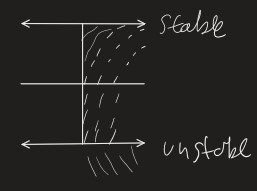
\includegraphics{resource/images/2.7 Example 1.jpg}
    \end{center}

    We need to classify each of the lines here as stable (a sink), unstable (a source), or semi-stable (a node). From this slope diagram we can make a phase diagram.

      

    The arrows in this diagram indicate whether $\frac{dy}{dx}$ is above or below $0$. We can see that the long term behavior of the solution:

    \[
      \begin{aligned}
        y_0 = y(t_0) > 2,\to y(t)\to 2\\
        - 2 < 2_0,\to y(t)\to 2\\
        y_0 <- 2, y(t)\to -\infty\\
      \end{aligned}
    \]
  \end{problem}

  Let's take a look at another example problem:

  \begin{problem}
    Compare the pivots of the two ordinary differential equations, $\frac{dy}{dt}=y^2(1-y)^2$, and $\frac{dy}{dx}=y^2(1-y^2)$.

    \begin{align*}
      \frac{dy}{dt}=y^2(1-y)^2 && \frac{dy}{dt}=y^2(1-y^2)\\
      0=y^2(1-y)^2 && 0=y^2(1-y^2)\\
      && y=0,\pm1\\
    \end{align*}
    From finding the equilibrium points of the differential equations, we can now craft a pivot diagram:\newline
    \begin{center}
    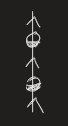
\includegraphics{resource/images/2.7 Example 2-1.jpg}
    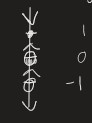
\includegraphics{resource/images/2.7 Example 2-2.jpg}
    \end{center}

    From this we can see that in the long term, the equations are going to look like this:

    \begin{align*}
      y_0<0,y(t)\to0\\
      0<y_0<1,y(t)\to1\\
      1<y_0,y(t)\to\infty\\
    \end{align*}
  \end{problem}

  \subsection{Bifurcations}

  For ordinary differential equations with a parameter, there are times that a small change in the value of the parameter results in a huge change in the behavior of the solutions. It causes a change in the number or stability of the equilibrium solutions.

  \begin{problem}
    Find the bifurcation value for 

    \[
      \frac{dp}{dt}=0.5p\left(1-\frac{p}{100}\right)-H
    \]

    The first step for finding a bifurcation for an equation is finding the equilibrium solutions. In order to do that, we set equation (2.69) equal to 0 and then rearrange it, so it is in the form

    \[
      p^2-100p+250H=0
    \]

    In this case, we are going to need to use the quadratic formula to find the equilibrium points:

    \begin{align*}
      p=\frac{100\pm\sqrt{10000-1000H}}{2}\\
      =50\pm5\sqrt{100-10H}
    \end{align*}
    We can determine that our bifurcation value is $H=10$, because if we take what's under the square root, and set it equal to zero we can find those values.
    Now we can plot our bifurcations:
    \begin{center}
      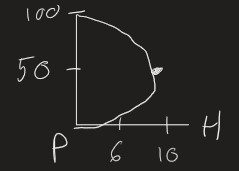
\includegraphics{resource/images/2.7 Example 3 1.jpg}
    \end{center}
  \end{problem}


\pagebreak

\medskip

\printbibliography[heading=bibintoc,title={\centering Bibliography}]

\end{document}
